\documentclass{article} % kind of document 
\usepackage[utf8]{inputenc} %encoding of choice
\usepackage[american]{babel} %language of choice
\usepackage[p,osf]{cochineal}
\usepackage{fancyhdr} %for header
\usepackage{amsmath, tabu} %math mode
\usepackage{mathtools}
\usepackage{extarrows} % for more options with arrows
\usepackage{amssymb} %math symbols
\usepackage{dsfont} %specifically for the indicator function symbol
\usepackage{xcolor} %to color text
\usepackage{amsthm} %math theorem
\usepackage{tikz}
\usepackage{caption}
\usepackage{multirow}
\usepackage[bottom]{footmisc}
% \usepackage[dvipsnames]{xcolor}
\usepackage{enumerate} %make lists
\usepackage{graphicx} %insert images
\usepackage{float} %to fix image position
\usepackage{moreverb} %to make boxes
\usepackage{hyperref} %to create hyperlinks
\usepackage{lipsum} %lorem ipsum package
\usepackage{setspace} % to use singlespace below in the solution environment
\usepackage[shortlabels]{enumitem}
\usepackage{parskip}
\usepackage[us]{datetime} %package for setting due date in US format
\newdate{duedate}{19}{10}{2021} %to set a due date
\allowdisplaybreaks
\usepackage[margin=1in]{geometry}
\pagestyle{fancy}
\usepackage{jlcode}

\lhead{Due: \displaydate{duedate}}
\chead{ECON 899 -- Problem Set 7 (SMM)}
\rhead{Danny, Hiroaki, Mitch, Ryan, Yobin}


\DeclareMathOperator*{\E}{\mathbb{E}} %ease of writing e and E
\newcommand{\e}{\mathrm{e}}
\newcommand{\ct}{\mathsf{c}}
\newcommand{\Z}{\mathbb{Z}}
\newcommand{\R}{\mathbb{R}}
\newcommand{\N}{\mathbb{N}}
\newcommand{\ifn}{\mathds{1}}
\newcommand{\X}{\mathbf{X}}
\newcommand{\Y}{\mathbf{Y}}
\newcommand{\one}{\mathbf{1}}
\newcommand\numberthis{\addtocounter{equation}{1}\tag{\theequation}}
\newcommand*\widebar[1]{\overline{#1}} % to get a widebar
\theoremstyle{definition}
\newtheorem{theorem}{theorem} % Theorem display format
\newtheorem{problem}[theorem]{Exercise} % Problem display format, last bracket sets display choice

\newenvironment{solution}[1][Answer]{\begin{singlespace}\underline{\textbf{#1:}}\quad }{\ \rule{0.3em}{0.3em}\end{singlespace}} % Answer format

\newenvironment{solutions}[1][Proof]{\begin{singlespace}\underline{\textbf{#1:}}\quad }{\ \rule{0.3em}{0.3em}\end{singlespace}} % Answer format

\begin{document}
	
	\begin{enumerate}
		\item Derive the following asymptotic moments associated with $ m_3(x) $ : mean, variance, first order auto-correlation. Furthermore, compute $ \nabla_b g(b_0) $. Which moments are informative for estimating $ b $?
		\begin{solution}
			We obtain the asymptotic moments as follows:
			\begin{align*}
				\E[x_t] & = \E[\rho_0 x_{t-1} + \epsilon_t] = \rho_0 \E[x_{t-1}] + \E[\epsilon_t] = \rho_0 \E[ \rho_0 x_{t-2} + \epsilon_{t-1} ] =  \rho_0^t \E[x_0] = 0.\\
				\E[(x_t - \E[x_t])^2] & = \E[x_t^2] = \E[(\rho_0 x_{t-1} + \epsilon_t)^2 ] \\ &= \rho_0^2 \E[x_{t-1}^2] + 2 \rho_0 \E[x_{t-1} \epsilon_t] + \E[\epsilon_t^2] \\ & = \rho_0^2 \E[ (\rho_0 x_{t-2} + \epsilon_{t-1})^2 ] + \sigma_0^2 \\ & = \rho_0^{2T} \E[x_0^2] + \sigma_0^2 \sum_{i=0}^{T-1} (\rho_0^2)^{i}  \rightarrow \frac{\sigma_0^2}{1 - \rho_0^2} = \frac{4}{3}.\\
				\E[(x_t - \E[x_t]) (x_{t-1} - \E[x_{t-1}]) ]&  =  \E[x_t x_{t-1}]  \\ &= \rho_0  \E[x_{t-1}^2]  + \E[ \epsilon_t x_{t-1} ] \\ & =   \rho_0 \E[ (\rho_0 x_{t-2} + \epsilon_{t-1})^2 ] \\ & =  \rho_0^3 \E[x_{t-2}^2] + \rho_0 \E[\epsilon_{t-1}^2]  \\ & = \rho_0^{2T - 1} \E[x_0^2] + \rho_0  \sigma_0^2 \sum_{i=0}^{T-2} (\rho_0^2)^{i}    \rightarrow  \frac{\rho_0 \sigma_0^2}{1 - \rho_0^2} = \frac{2}{3}   \\
			\end{align*}
			Moreover, we have that $ \nabla_b =
				\renewcommand\arraystretch{1.6}
			\begin{pmatrix}
				\frac{\partial}{\partial \rho} \\
				 \frac{\partial}{\partial \sigma^2}
			\end{pmatrix} $. Evaulating the derivative of $ g(\cdot) $ at $ b = b_0 $ gives us
			\begin{align*}
				\nabla_b g(b_0) = 
				\renewcommand\arraystretch{2}
				\begin{bmatrix}
					0 & 0 \\ \frac{2 \rho_0 \sigma_0^2}{(1 - \rho_0)^2} & \frac{1}{1 - \rho_0^2} \\  \frac{\sigma_0^2( 1 + 2 \rho_0^2)}{(1 - \rho_0^2)^2}  & \frac{\rho_0}{1 - \rho_0^2}
				\end{bmatrix}
				\xlongequal{\text{true values}}
				\begin{bmatrix}
					0 & 0 \\  4 & \frac{4}{3} \\  \frac{8}{3} & \frac{2}{3}
				\end{bmatrix}
			\end{align*}
		
			Both the variance and the first order correlation are informative for estimating $ b $. This is because we can estimate the true parameters given the two moments as follows
			\begin{align*}
				\rho_0 = \frac{ \E[(x_t - \E[x_t]) (x_{t-1} - \E[x_{t-1}]) ] }{ 	\E[(x_t - \E[x_t])^2]  } && \sigma^2 =  \E[(x_t - \E[x_t])^2] -  \frac{ \E[(x_t - \E[x_t]) (x_{t-1} - \E[x_{t-1}]) ] }{ 	\E[(x_t - \E[x_t])^2]  }
			\end{align*}
		\end{solution}
		\item Simulate a series of “true” data of length $ T = 200 $ using (1). We will use this to compute
		$ M_T (x) $.
		
		\item Set H = 10 and simulate H vectors of length T = 200 random variables $ e_t $ from $ N(0, 1) $. We will use this to compute $ M_{TH}(y(b)) $. Store these vectors. You will use the same vector of random variables throughout the entire exercise. Since this exercise requires you to estimate $ \sigma^2 $, you want to change the variance of $ e_t $ during the estimation. You can simply use $ \sigma_{e_t} $ when the variance is $ \sigma^2 $.
		\item We will start by estimating the$l = 2$ vector $b$ for the just identified case where $m_{2}$ uses mean and variance. Given what you found in part (1), do you think there will be a problem? Of course, in general we would not know whether this case would be a problem, so hopefully the standard error of the estimate of $b$ as well as the $J$ test will tell us something. Let’s see.
		\begin{solution}
		The code for completing this question, as well as the other questions for this problem set, is included in the appendix. From the results of part (1), we know that the mean will be uninformative about the true parameter values, and so in this case only the variance will be useful in identifying the parameter values. One problem that we notice here and elsewhere is that occasionally the random draws selected by the code will produce issues like negative values for variance. \textbf{COME BACK TO THIS AND DOUBLE CHECK} In this problem and for the remainder of the problem set, then, we set specific random seed values to avoid this issue. These values are shown in the code.
		\begin{enumerate}[label=(\alph*)]
			\item $\hat{b}_{TH}^{1}=[0.7178,0.855]$. Figure \ref{4a} displays a graph of the objective function.
			\begin{figure}[htbp] 
				\centering
				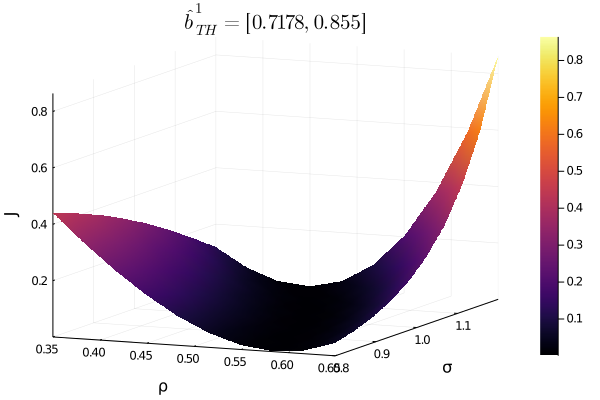
\includegraphics[scale=.5]{Figures/Exercise4.png}
				\caption{Objective Function for Exercise 4 \label{4a}}
			\end{figure}
			\item $\hat{b}_{TH}^{2}=[0.7179,0.8549]$ after the Newey-West correction. Figure \ref{4b} displays a graph of the objective function.
			\begin{figure}[htbp] 
				\centering
				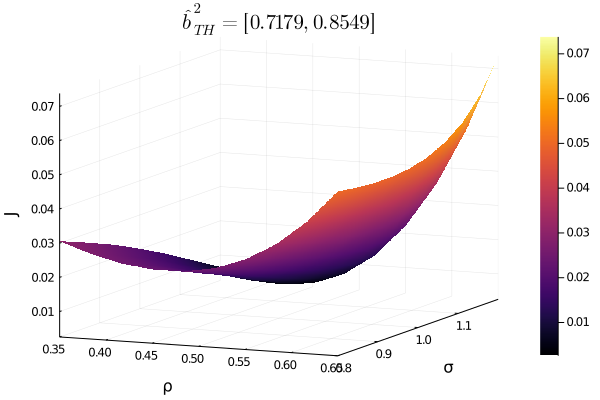
\includegraphics[scale=.5]{Figures/Exercise4NeweyWestCorrection.png}
				\caption{Opbjective Function for Exercise 4 with the Newey-West Correction \label{4b}}
			\end{figure}
			\item
				\begin{equation*}
					\nabla_{b} g_{T}(\hat{b}^{2}_{TH})=\begin{bmatrix}
											0.22 & 0.06 \\
											3.66 & 3.11
											\end{bmatrix}
				\end{equation*}
				The variance-covariance matrix of $\hat{b}^{2}_{TH}$ is given by
				\begin{equation*}
											\begin{bmatrix}
											0.01 & -4.07e-3 \\
											-4.07e-3 & 0.01
											\end{bmatrix}
				\end{equation*}
				The standard errors are given by
				\begin{equation*}
											\begin{bmatrix}
											0.08 \\
											0.11
											\end{bmatrix}
				\end{equation*}
				For local identification, it is useful to have the elements of $\nabla_{b} g_{T}(\hat{b}^{2}_{TH})$ to be relatively large. This is because if the distance between the modeled moments and the data moments is changing rapidly around the optimal parameter choices, we can be more confident in the precision with which we've identified the local optimal parameter values.
			\item The $J$-test value is $1.17e-6$.
		\end{enumerate}
		\end{solution}
		\item Next we estimating the $ l = 2 $ vector $ b $ for the just identified case where $ m_2 $ uses the variance and autocorrelation. Given what you found in part (1), do you now think there will be a problem? If not, hopefully the standard error of the estimate of $ b $ as well as the J test will tell us something. Let’s see. For this case, perform steps (a)-(d) above.
		\begin{solution}
		Given our results from part (1), we know that the variance and first order correlation are both informative for estimating $b$. Therefore, we do not anticipate a major problem here.
		\begin{enumerate}[label=(\alph*)]
			\item $\hat{b}_{TH}^{1}=[0.4408,1.0751]$. Figure \ref{5a} displays a graph of the objective function.
			\begin{figure}[htbp] 
				\centering
				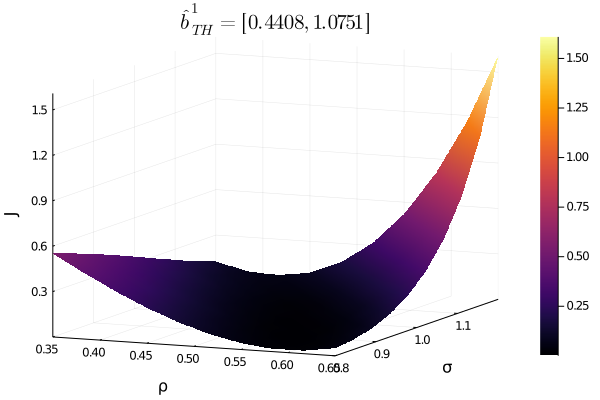
\includegraphics[scale=.5]{Figures/Exercise5.png}
				\caption{Objective Function for Exercise 5 \label{5a}}
			\end{figure}
			\item $\hat{b}_{TH}^{2}=[0.4409,1.075]$ after the Newey-West correction. Figure \ref{5b} displays a graph of the objective function.
			\begin{figure}[htbp] 
				\centering
				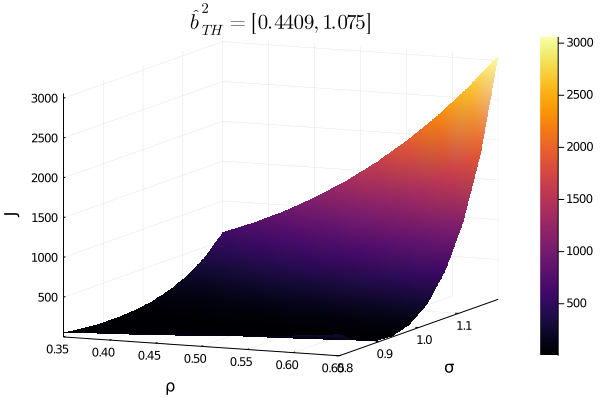
\includegraphics[scale=.5]{Figures/Exercise5NeweyWestCorrection.png}
				\caption{Opbjective Function for Exercise 5 with the Newey-West Correction \label{5b}}
			\end{figure}
			\item
				\begin{equation*}
					\nabla_{b} g_{T}(\hat{b}^{2}_{TH})=\begin{bmatrix}
											1.44 & 2.78 \\
											1.83 & 1.22
											\end{bmatrix}
				\end{equation*}
				The variance-covariance matrix of $\hat{b}^{2}_{TH}$ is given by
				\begin{equation*}
											\begin{bmatrix}
											7.43e-5 & -1.02e-3 \\
											-1.02e-3 & 0.01
											\end{bmatrix}
				\end{equation*}
				The standard errors are given by
				\begin{equation*}
											\begin{bmatrix}
											0.01 \\
											0.12
											\end{bmatrix}
				\end{equation*}
				For local identification, it is useful to have the elements of $\nabla_{b} g_{T}(\hat{b}^{2}_{TH})$ to be relatively large. This is because if the distance between the modeled moments and the data moments is changing rapidly around the optimal parameter choices, we can be more confident in the precision with which we've identified the local optimal parameter values.
		\end{enumerate}
		\end{solution}
		
		\item Next, we will consider the overidentified case where m3 uses the mean, variance and autocorrelation. Let’s see. For this case, perform steps (a)-(d) above. Furthermore, bootstrap the the finite sample distribution of the estimators using the following algorithm:
		\begin{enumerate}[i.]
			\item Draw $ \epsilon_t $ and $ e_t^h $ from $ N(0,1) $ for $ t = 1,2,\hdots,T $ and $ h = 1,2,\hdots,H $. Compute $ (\hat{b}_{TH}^1), \hat{b}_{TH}^2 $ as described.
			
			\item Repeat (e) using another seed.
		\end{enumerate}
	
	\end{enumerate}

	\section*{Appendix}
 	The first codefile named "RunCode.jl" runs the code.
 	\jlinputlisting{Code/RunCode.jl}
	
 	The second codefile named "Code.jl" contains the relevant functions.
 	\jlinputlisting{Code/Code.jl}
\end{document}